\documentclass[letterpaper]{article}
\usepackage[utf8]{inputenc}
%\usepackage[latin1]{inputenc}
\usepackage[spanish]{babel}
\usepackage{geometry}
\usepackage{anysize}
\usepackage{graphicx}
\usepackage{float} 
\usepackage{amsmath}
\usepackage{lscape}
%\numberwithin{equation}{list}
\marginsize{1cm}{2cm}{0cm}{2cm}  
\title{Evaluación Tema 3 \\ \begin{large}Curso de Física Computacional\end{large}}
\author{M. en C. Gustavo Contreras Mayén}
\date{ }
\begin{document}
%\begin{landscape}
\maketitle
\fontsize{10}{10}\selectfont
\spanishdecimal{.}
\begin{flushright}
Fecha: \line(1,0){20} / \line(1,0){20} /\line(1,0){20}
\end{flushright}
Nombre: \underline{Ricardo Saúl García Jiménez}.
\\
\\
\fontsize{14}{14}\selectfont
Para todos los problemas se pidió que considerasen los atributos que se evalúan en la rúbrica, y la siguiente fue la que entregaste el día de revisión del examen, que fue el 24/4/2014.
\fontsize{10}{10}\selectfont
\begin{center}
\renewcommand{\arraystretch}{2.5}
\begin{tabular}{| l | c | c | c | c | c | c | c | c |}
\hline
 & Documentación & Modularidad & Eficiencia & Robustez & Graficación & Ejecución & Interpretación & Suma \\ \hline
Problema 1 & 2 & 3 & 3 & 3 & 2 & 3 & 2 & 18 \\ \hline
Problema 2 & 2 & 3 & 3 & 3 & 2 & 3 & 2 & 18 \\ \hline
Problema 3 & 2 & 3 & 3 & 3 & 2 & 3 & 2 & 18 \\ \hline
Problema 4 & 2 & 3 & 3 & 3 & 2 & 3 & 2 & 18 \\ \hline
Problema 5 & 2 & 3 & 3 & 3 & 2 & 3 & 2 & 18 \\ \hline
Problema 6 & 2 & 3 & 3 & 3 & 2 & 3 & 2 & 18 \\ \hline
Problema 7 & 2 & 3 & 3 & 3 & 2 & 3 & 2 & 18 \\ \hline
Problema 8 & 2 & 3 & 3 & 3 & 2 & 3 & 3 & 19 \\ \hline
\end{tabular}
\end{center}
\fontsize{14}{14}\selectfont
A continuación, se detalla la puntuación para cada atributo de la rúbrica.
\\
\\
\textbf{Documentación:}
\begin{itemize}
\item \emph{Excepcional, 3 puntos:} El programa contiene documentación extensa, incluyendo el nombre de quien programó, describe la operación del todo el programa, así como detalla la operación de cada función/módulo
\item \emph{Aceptable, 2 puntos:} Cuenta con información sobre lo que realiza el programa, pero sin llegar a detallar cada uno de los componentes incluidos en el código.
\item \emph{Novato, 1 punto:} Se incluye poca información sobre el programa y lo que realiza.
\item \emph{No satisfactorio, 0 puntos:} Carece completamente de documentación.
\end{itemize}
Para los ocho problemas, dado que no cuenta con ningún tipo de documentación que refiera lo qué hace el código, alguna modificación siquiera a parámetros, como podrás revisar en los archivos que me entregaste, no hay documentación alguna, por lo que en este rubro, la evalución del profesor a diferencia de la que haces tu, queda en 0 puntos.
\\
\\
Para los atributos de Modularidad, Eficiencia y Robustez, se usaron los mismos módulos que construimos en clase, no hay alguno nuevo o modificado; siempre tuvieron la libertad de crear sus propias rutinas, módulos o funciones. El que se re-utilicen es bueno, pero no necesariamente quiere decir que se evalúe como una aportación propia, te calificas con 3 puntos para cada problema en los atributos mencionados, la evaluación del profesor queda en 2 puntos.
\\
\\
\textbf{Graficación:}
\begin{itemize}
\item \emph{Excepcional, 3 puntos:} El programa genera gráficas que representan el resultado obtenido del problema, cuentan con información detallada en ejes, título, leyendas, colores marcadores para las curvas, incluyendo el manejo de subgráficas.
\item \emph{Aceptable, 2 puntos:} El programa genera gráficas que representa el resultado del problema, la información no es tan detallada, se manejan diferentes gráficas de manera separada.
\item \emph{Novato, 1 punto:} El programa genera gráficas que representan el resultado del problema, no cuentan con identificadores de ningún tipo.
\item \emph{No satisfactorio, 0 puntos:} El programa no genera ningún tipo de gráfica.
\end{itemize}
Para el problema 1:
\begin{figure}[H]
	\centering
	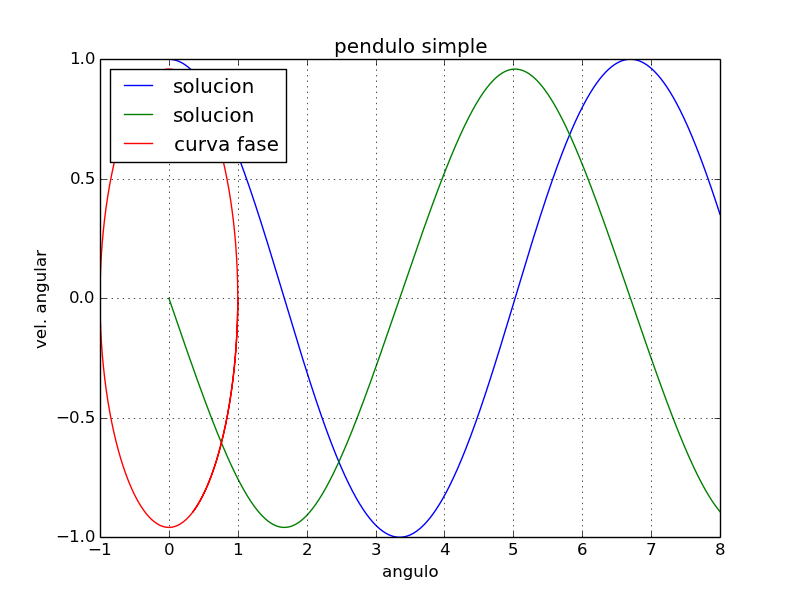
\includegraphics[scale=0.5]{Problema1_Ricardo.png} 
\end{figure}
Para el problema 2:
\begin{figure}[H]
	\centering
	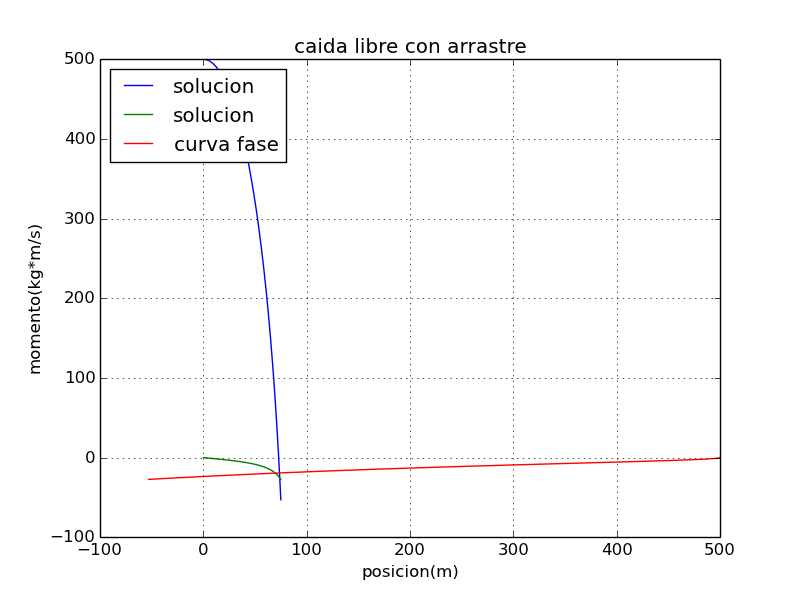
\includegraphics[scale=0.5]{Problema2_Ricardo.png} 
\end{figure}
Para el problema 3:
\begin{figure}[H]
	\centering
	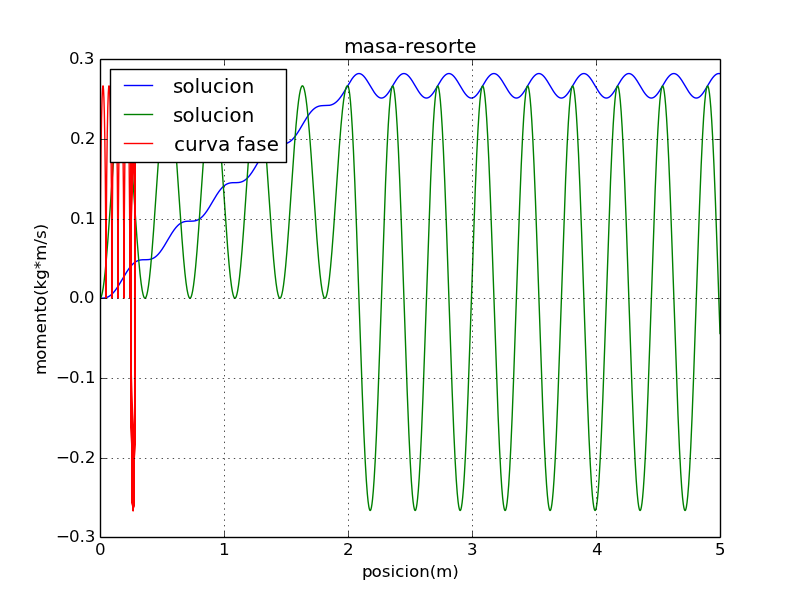
\includegraphics[scale=0.5]{Problema3_Ricardo.png} 
\end{figure}
Para el problema 4:
\begin{figure}[H]
	\centering
	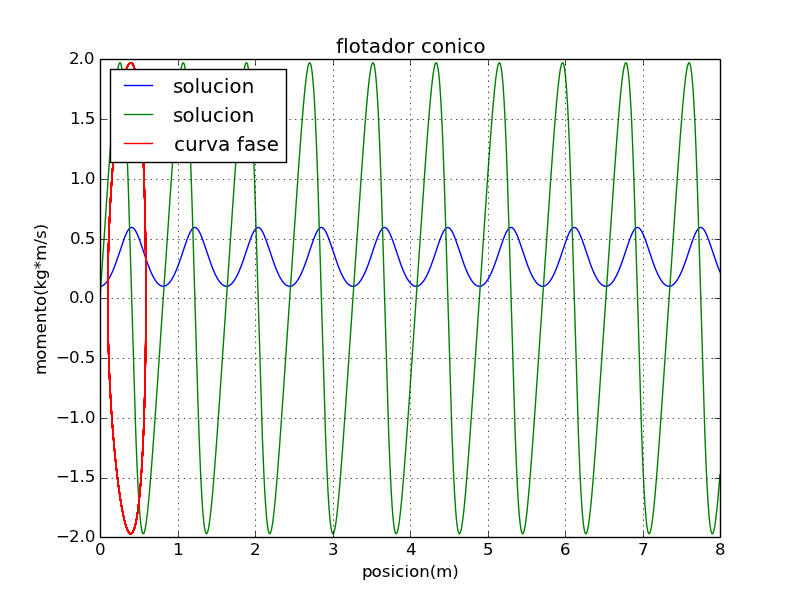
\includegraphics[scale=0.5]{Problema4_Ricardo.png} 
\end{figure}
Para el problema 5:
\begin{figure}[H]
	\centering
	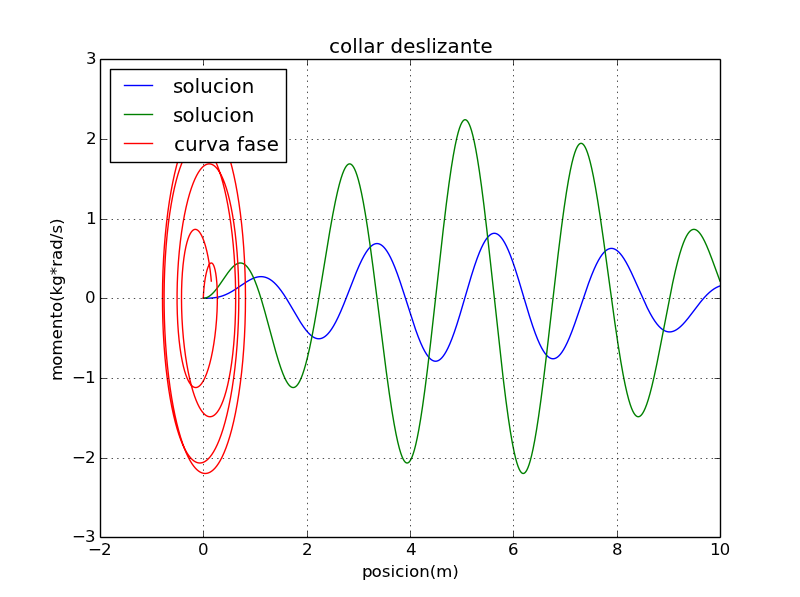
\includegraphics[scale=0.5]{Problema5_Ricardo.png} 
\end{figure}
Para el problema 6:
\begin{figure}[H]
	\centering
	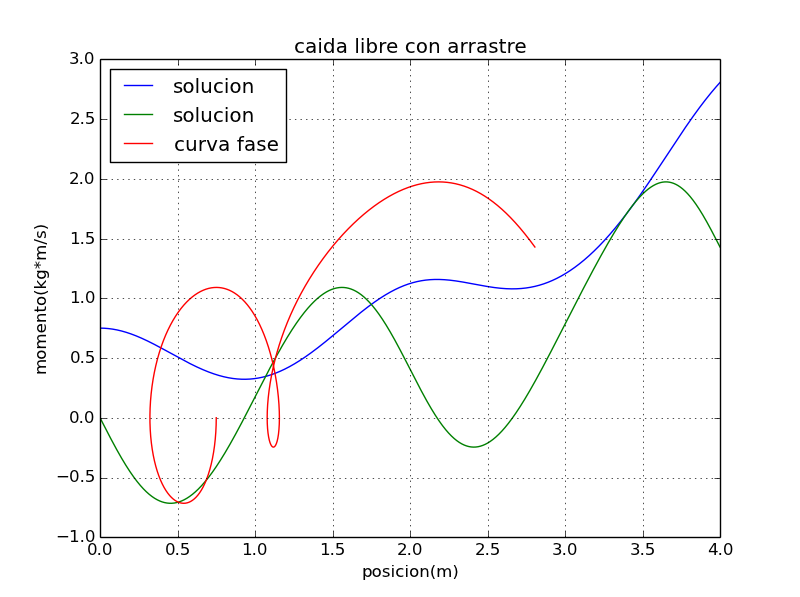
\includegraphics[scale=0.5]{Problema6_Ricardo.png} 
\end{figure}
Para el problema 7:
\begin{figure}[H]
	\centering
	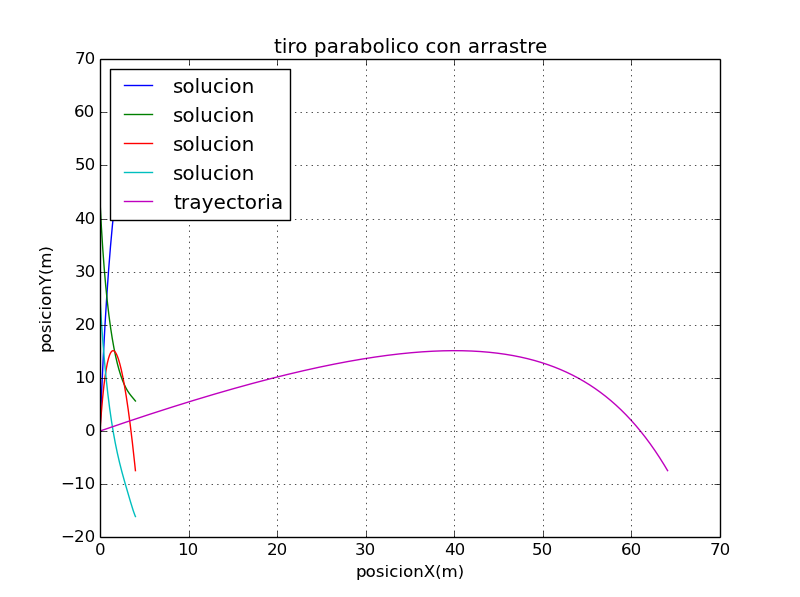
\includegraphics[scale=0.5]{Problema7_Ricardo.png} 
\end{figure}
Para el problema 8:
\begin{figure}[H]
	\centering
	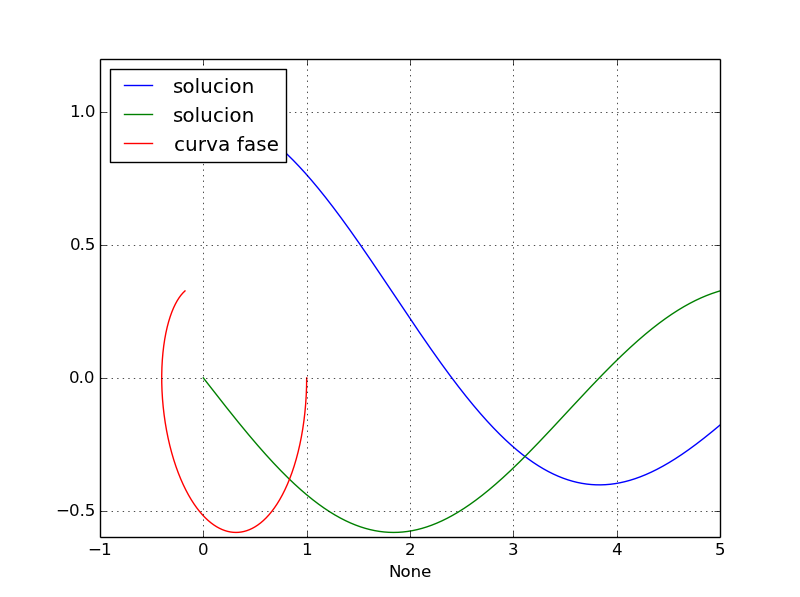
\includegraphics[scale=0.5]{Problema8_Ricardo.png} 
\end{figure}
Como podrás revisar, cada una de las gráficas no separa la gráfica del espacio fase, las etiquetas de cada curva no están identificadas, por lo que no se sabe qué se está graficando, en el código sabemos que se trabaja con y' y con y, pero en tu resultado visual, debe de tener la claridad sobre el resultado, y para cada problema, va muy de la mano con el atributo de la interpretación en la solución, que para cada ejercicio, no se da interpretación alguna.
\\
\\
Te evalúas con 2 puntos, la evaluación del profesor es de 1 puntos para cada problema.
\\
\\
En el atributo de Ejecución, es similar al de los de Modularida, Eficiencia y Robustez, ya que el código reutilizado fue el que trabajamos en clase, por tanto, había la garantía de que todo estaría funcionando bien, te evaluaste con 3 puntos, la evaluación del profesor es de 2 puntos.
\\
\\
\textbf{Interpretación:}
\begin{itemize}
\item \emph{Excepcional, 3 puntos:} El problema se entrega con una interpretación extensa apoyándose en los elementos que el mismo código genera, discute la posibilidad de resultados, modificación de parámetros, contrasta contra el fenómeno físico o matemático.
\item \emph{Aceptable, 2 puntos:} El problema se entrega con una interpretación que se apoya con los elementos que genera el mismo código.
\item \emph{Novato, 1 punto:} El problema se entrega con una interpretación de  resultados muy vaga: se reporta un resultado sin explicación.
\item \emph{No satisfactorio, 0 puntos:} El problema a resolver se entrega sin una interpretación de los resultados obtenidos, sólo se entrega el código.
\end{itemize}
Te evaluaste con 2 puntos y en el caso del problema 8, hasta con 3 puntos. Pero no encuentro en ninguna parte de tu código esa interpretación, se pidió en clase que la interpretación corresponde a correlacionar el resultado que devuelve el código, apoyándose con las gráficas, haciendo modificaciones a parámetros, todo ello, contra el fenómeno físico. Entonces, para este atributo, la calificación para cada problema es cero.
\\
\\
Por la razones anteriormente expuestas, la calificación de tu examen es 7 (siete), no basta con haber entregado todos los ejercicios, sino el trabajo que implica usar un código que en gran parte ya se había desarrollado en clase; si hubieran sido 20 problemas en el examen, cada uno de ellos, se evaluaría con los atributos de la rúbrica.
%\end{landscape}
\end{document}